\documentclass[conference]{IEEEtran}
\usepackage{color}
\usepackage{tikz}

% Terri's simple FIXME macro
\newcommand{\FIXME}[1]{\textcolor{red}{FIXME: #1}}

% Tikz setup
\usetikzlibrary{arrows,decorations,decorations.text,decorations.pathreplacing,shapes}
\tikzstyle{box} = [rectangle, draw, text width=8em]
\tikzstyle{thread} = [rectangle, draw, minimum width=1em, minimum height=1em, fill=blue!40]
\tikzstyle{thread-cloud} = [cloud, draw, cloud puffs=10,cloud puff arc=120, aspect=2, inner ysep=1em, minimum width=16em, minimum height=12em]

\begin{document}
\title{Automated Proactive Software Hardening\\ through Fuzz Testing and Evolutionary Computation}

\author{}
%\author{\IEEEauthorblockN{Michael Shell}
%\IEEEauthorblockA{School of Electrical and\\Computer Engineering\\
%Georgia Institute of Technology\\
%Atlanta, Georgia 30332--0250\\
%Email: http://www.michaelshell.org/contact.html}
%\and
%\IEEEauthorblockN{Homer Simpson}
%\IEEEauthorblockA{Twentieth Century Fox\\
%Springfield, USA\\
%Email: homer@thesimpsons.com}
%\and
%\IEEEauthorblockN{James Kirk\\ and Montgomery Scott}
%\IEEEauthorblockA{Starfleet Academy\\
%San Francisco, California 96678-2391\\
%Telephone: (800) 555--1212\\
%Fax: (888) 555--1212}}

\maketitle

\begin{abstract}
Hardening software to make it more robust and able to withstand attacks can be
very challenging.  This paper explores a method for automated hardening by
combing an automated bug-finding technique with automated software
repair in a closed loop automated software hardening tool.  We
demonstrate the effectiveness of this approach through proactive
defeat of withheld real-world exploits.
\end{abstract}

\section{Introduction}
In their 2006 paper, Miller et al were disappointed to find that the robustness
of command line utilities on MacOS in 2006 than the Linux/GNU tools of 1995
\cite{Miller2006}.  While fuzz testing is a well-established technique for
testing software robustness, applying it to an existing project and then fixing
the bugs found as a result of this techinque takes time.  Unfortunately,
developers already can find more bugs than they realistically have time to fix
\cite{devshavetoomanybugs}.  \FIXME{blah blah about bugs, use citations from
previous genprog papers.}

However, it is now possible to use automted repair to fix bugs rather than
relying on human programmers.  This has proven to be very competitive, with one
study finding that bugs could be repaired for approximately \$8 per bug
\cite{manybugs}. \FIXME{some paragraph about genprog here, or maybe later?}

So we have an automated way to find bugs and an automated way to fix them: is it
possible to combine the two to proactively ``harden" software? 


\section{Technical Approach}

\begin{figure*}[htb]
  \centering
  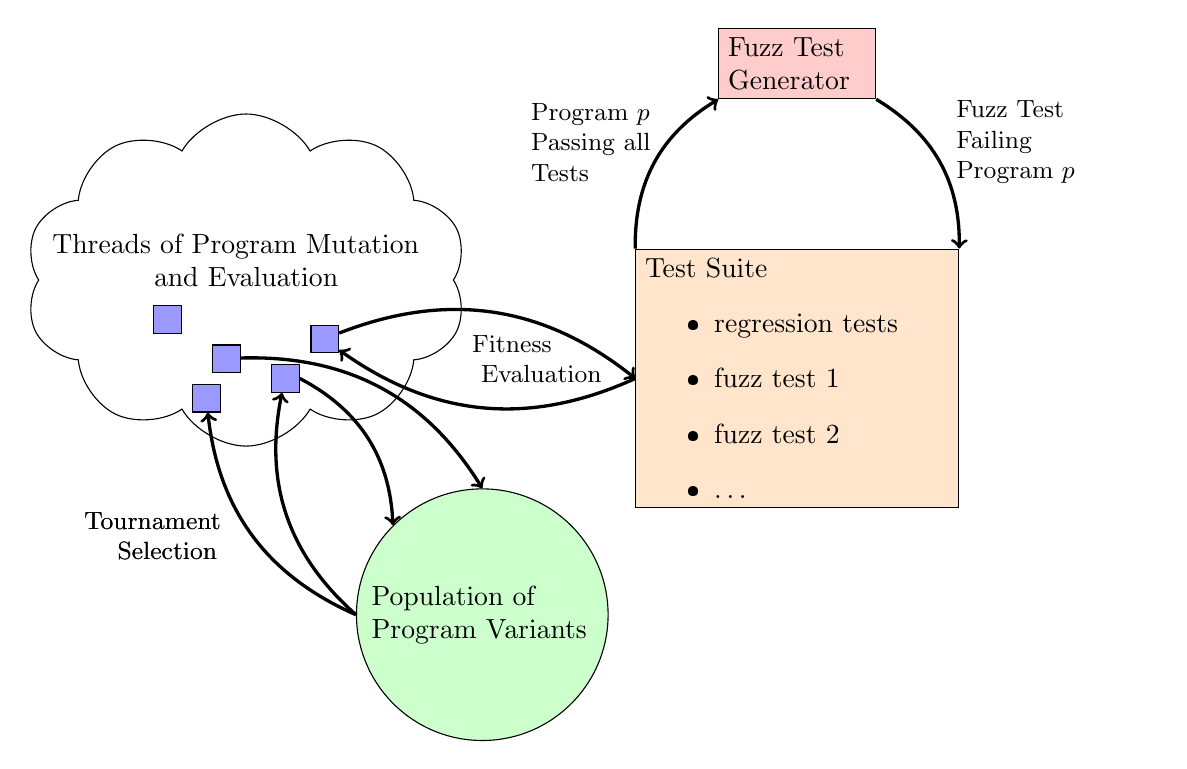
\begin{tikzpicture}[scale=0.5]
    \node [box, fill=red!20, text width=5em] (fuzz) at (6,2) {Fuzz Test\\Generator};
    \node [text width=14em] (genprog) at (-8,-3) {Threads of Program Mutation\\\centerline{and Evaluation}};
    \node [box, circle, fill=green!20] (pop) at (-2,-12) {Population of\\ Program Variants};
    \node [box, text width=11em, fill=orange!20] (test) at (6, -6)
    {Test Suite
      \begin{itemize}
      \item regression tests
      \item fuzz test 1
      \item fuzz test 2
      \item \ldots{}
      \end{itemize}};
    \node [thread-cloud] at (-8,-3.5) {};
    \node [thread] (t1) at (-9,-6.5) {};
    \node [thread] (t2) at (-7,-6) {};
    \node [thread] (t3) at (-6,-5) {};
    \node [thread] (t4) at (-10,-4.5) {};
    \node [thread] (t5) at (-8.5,-5.5) {};

    % population <-> threads
    \draw [->,very thick,bend left] (pop.west) to (t1);
    \draw [->,very thick,bend left] (pop.west) to (t2);
    \draw [->,very thick,bend left] (t5) to (pop.north);
    \draw [->,very thick,bend left] (t2.east) to (pop.north west);
    % threads <-> test
    \draw [->,very thick,bend left] (t3) to (test.west);
    \draw [->,very thick,bend left] (test.west) to (t3);
    % test <-> fuzz generator
    \draw [->,very thick,bend left] (test.north west) to (fuzz.south west);
    \draw [->,very thick,bend left] (fuzz.south east) to (test.north east);

    % arrow labels
    \node [text width=6em, font=\small] at (-10,-10) {Tournament\\\centerline{Selection}};
    \node [text width=6em, font=\small] at (-10,-10) {Tournament\\\centerline{Selection}};
    \node [text width=5em, font=\small] at (-0.5,-5.5) {Fitness\\\centerline{Evaluation}};
    \node [text width=5em, font=\small] at (1,0) {Program $p$ Passing all Tests};
    \node [text width=7em, font=\small] at (12.5,0) {Fuzz Test\\Failing\\Program $p$};
  \end{tikzpicture}
  
  \caption{Overview of Fuzz Hardening framework}
  \label{fig:overview}
\end{figure*}

\subsection{Fuzz Testing}

Fuzz testing is a fairly mature technique that can range from the original work
using purely random characters \cite{Miller1990,Miller1995} to input that is
very specifically tweaked from a template or grammar \cite{modern,fuzz,papers}, or
randomized input that includes mouse or window events \cite{Miller2006}.

For our experiments, we've started with the most basic fuzz tester,
as provided by Miller as fuzz-2001 \cite{Millerfuzzwebsite}, which generates
different lengths of files filled with randomized characters.   The system has
been designed so that this piece can be replaced with a more advanced fuzz
tester if one is available for the program in question.  However, we were
curious if even a fairly modest fuzzer could be used to produce useful software
hardening, and this is the most basic of those available.

\subsection{Automated Software Repair}

For the automated software repair part of the system, we have used a lisp
implementation of Genprog \cite{genprogpapers}.   This particular version of
genprog was easier to script for repeated repairs.  \FIXME{more here}



\section{Conclusion}
The conclusion goes here.

\section*{Acknowledgment}

The authors would like to thank...
- DARPA

\bibliographystyle{IEEEtran}
\bibliography{pst2013.bib}

\end{document}
